\documentclass[conference]{IEEEtran}

\usepackage{cite}
\usepackage{amsmath,amssymb,amsfonts}
\usepackage{graphicx}
\usepackage{textcomp}
\usepackage{xcolor}
\usepackage{booktabs}
\usepackage{multirow}
\usepackage{url}
\usepackage{tikz}
\usetikzlibrary{positioning,arrows.meta,shapes.geometric,fit,backgrounds}

\graphicspath{{../figures/}{../checkpoints/baseline_v2/}{../checkpoints/baseline_v2/robustness/}}

\begin{document}

\title{Robust Contactless Palmprint Verification with Deep Metric Learning:\\Checkpoint 2 --- Advanced Model, Baseline Comparison, and Robustness Analysis}

\author{
\IEEEauthorblockN{Huy Ong}
\IEEEauthorblockA{CS 228 -- Biometric Security\\Spring 2026}
}

\maketitle

\begin{abstract}
Checkpoint~1 established the data foundation and an initial ResNet18 + ArcFace embedding model for contactless palmprint verification. Checkpoint~2 takes a technical deep dive: we present a full system architecture, expand the methodology with formal loss and scoring definitions, survey 5--7 related state-of-the-art methods, and benchmark the advanced model against a realistic baseline floor. On the PolyU--IITD dataset (611 subjects, 12{,}220 images, subject-disjoint splits), our advanced model reaches an Equal Error Rate (EER) of 1.67\% on clean test data, a 3.9$\times$ reduction over an ImageNet-pretrained ResNet18 baseline (EER 6.50\%). A systematic benchmark across 9 corruption types $\times$ 5 severity levels exposes critical vulnerabilities: noise (+1{,}170\% EER), motion blur (+1{,}041\%), and brightness shifts (+796\%) cause the steepest drops, while contrast and scale changes remain tractable. These targeted weaknesses motivate the mitigation work planned for the final phase.
\end{abstract}

% ============================================================
\section{Refined Problem Statement}

As established in Checkpoint~1, this project investigates the robustness of a deep learning--based palmprint verification system to common capture variations. Checkpoint~2 extends that work by (i) formalizing the full system architecture, (ii) articulating the mathematical formalism of the training objective and matcher, (iii) comparing the advanced model to a quantitative baseline floor, and (iv) presenting a full robustness benchmark.

\subsection{Scope Changes Since Checkpoint 1}

{\color{blue}
\begin{itemize}
    \item \textbf{Dropped:} MobileNetV3 backbone comparison---effort was reinvested in a thorough robustness benchmark and a rigorous baseline floor.
    \item \textbf{Added:} An ImageNet-pretrained-only ResNet18 \emph{baseline floor} (no fine-tuning) scored on the identical test pair set, providing a concrete non-trivial reference point.
    \item \textbf{Completed:} Full robustness benchmark across 9 corruption types $\times$ 5 severity levels (45 conditions), exceeding the originally planned 4--6 types.
    \item \textbf{Deferred:} Mitigation (robust augmentation training or quality gating) is deferred to the final phase.
\end{itemize}
}

% ============================================================
\section{System Architecture}
\label{sec:arch}

Fig.~\ref{fig:arch} diagrams the end-to-end verification pipeline, with the five labeled stages required of a biometric system: input interface, preprocessing pipeline, feature extraction and template generation, matcher, and database store.

\begin{figure*}[t]
\centering
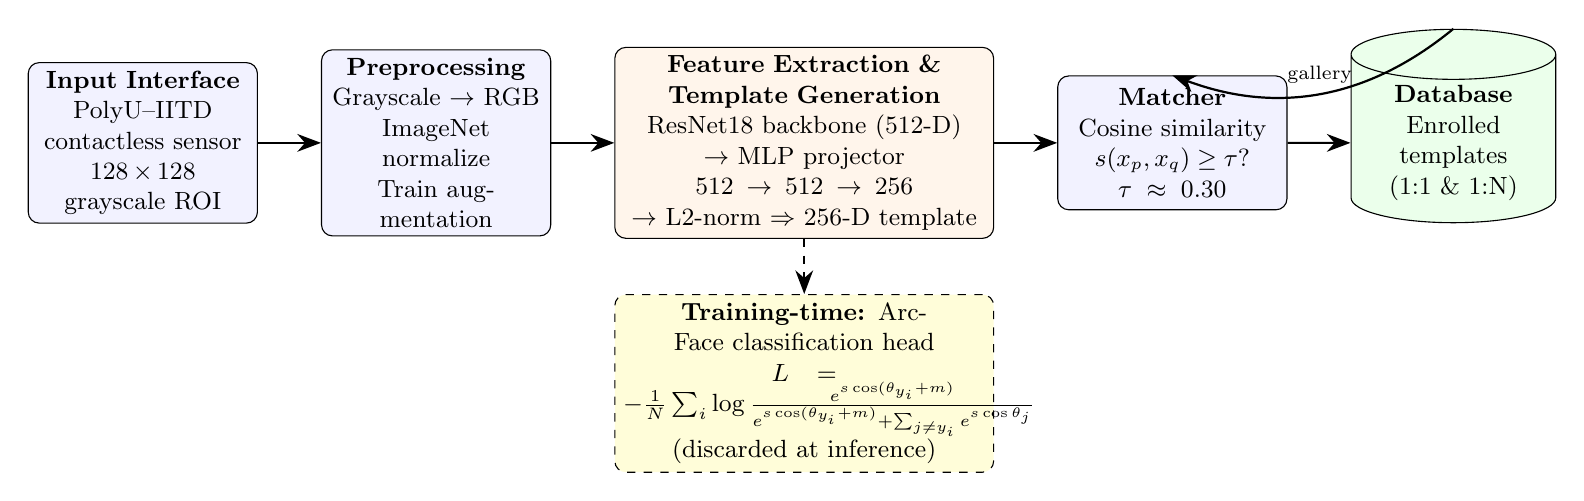
\begin{tikzpicture}[
    font=\small,
    every node/.style={align=center},
    box/.style={draw, rounded corners, minimum height=1.7cm, minimum width=2.6cm,
                text width=2.7cm, inner sep=3pt, fill=blue!5},
    bigbox/.style={draw, rounded corners, minimum height=1.7cm, minimum width=4.6cm,
                   text width=4.6cm, inner sep=3pt, fill=orange!8},
    store/.style={draw, cylinder, shape border rotate=90, aspect=0.25,
                  minimum height=1.7cm, minimum width=2.6cm, text width=2.4cm,
                  inner sep=2pt, fill=green!8},
    lossbox/.style={draw, dashed, rounded corners, fill=yellow!15, text width=4.6cm,
                    inner sep=3pt},
    arr/.style={-{Stealth[length=3mm]}, thick},
]

% Stage boxes
\node[box]    (input)    {\textbf{Input Interface}\\PolyU--IITD contactless sensor\\$128\!\times\!128$ grayscale ROI};
\node[box, right=0.8cm of input]   (pre)   {\textbf{Preprocessing}\\Grayscale $\to$ RGB\\ImageNet normalize\\Train augmentation};
\node[bigbox, right=0.8cm of pre]  (feat)  {\textbf{Feature Extraction \& Template Generation}\\ResNet18 backbone (512-D)\\$\to$ MLP projector $512\!\to\!512\!\to\!256$\\$\to$ L2-norm $\Rightarrow$ 256-D template};
\node[box, right=0.8cm of feat]    (match) {\textbf{Matcher}\\Cosine similarity\\$s(x_p,x_q)\!\geq\!\tau$?\\$\tau\approx 0.30$};
\node[store, right=0.8cm of match] (db)    {\textbf{Database}\\Enrolled\\templates\\(1:1 \& 1:N)};

% Training-time loss block (below feature extractor)
\node[lossbox, below=0.7cm of feat] (loss) {\textbf{Training-time:} ArcFace classification head\\$L = -\tfrac{1}{N}\sum_i \log \tfrac{e^{s\cos(\theta_{y_i}+m)}}{e^{s\cos(\theta_{y_i}+m)} + \sum_{j\neq y_i} e^{s\cos\theta_j}}$\\(discarded at inference)};

% Arrows
\draw[arr] (input)  -- (pre);
\draw[arr] (pre)    -- (feat);
\draw[arr] (feat)   -- (match);
\draw[arr] (match)  -- (db);
\draw[arr, dashed] (feat) -- (loss);

% Bi-directional between matcher and store (enrollment / query)
\draw[arr] (db.north) to[bend left=30] node[above]{\scriptsize gallery} (match.north);

\end{tikzpicture}
\caption{System architecture for palmprint verification. Input images are normalized and passed through a ResNet18 backbone and projection head that produce L2-normalized 256-D templates. At enrollment, templates are stored in the database; at verification, a query template is compared against a gallery entry via cosine similarity and thresholded. The ArcFace classification head (dashed) is used only during training to structure the embedding space and is discarded at inference.}
\label{fig:arch}
\end{figure*}

\paragraph{Input interface}
Raw input is the PolyU--IITD contactless palmprint sensor output, pre-cropped to $128\!\times\!128$ grayscale ROI.

\paragraph{Preprocessing pipeline}
Grayscale frames are expanded to 3-channel RGB for ImageNet-pretrained backbones and normalized with ImageNet channel statistics. During training, augmentation (random crop, horizontal flip, $\pm 15^\circ$ rotation, color jitter, Gaussian blur, random erasing) reduces overfitting.

\paragraph{Feature extraction \& template generation}
A ResNet18 backbone extracts 512-D features; a two-layer MLP projector with batch normalization and ReLU reduces this to a 256-D embedding; L2 normalization places the template on the unit hypersphere, making cosine similarity the natural matcher score.

\paragraph{Matcher/Classifier}
At inference, two templates $f(x_p)$, $f(x_q)$ are compared by cosine similarity; a decision threshold $\tau$ (set at the EER operating point, $\tau \approx 0.30$) decides accept or reject. At training time, an ArcFace classification head~\cite{deng2019arcface} with scale $s\!=\!30$, margin $m\!=\!0.3$, imposes an angular margin between classes to sharpen inter-identity separation.

\paragraph{Database store}
Enrolled templates are indexed by (subject, hand) class label. The store supports 1:1 verification (one gallery template per claim) and 1:N identification (rank all gallery templates by similarity).

% ============================================================
\section{Data Engineering}

\subsection{Dataset Recap}
We use the PolyU--IITD Contactless Palmprint Database v3.0~\cite{polyu} with 611 subjects (12{,}220 images), subject-disjoint splits (427/61/123 train/val/test), and each (subject, hand) pair as a unique class. Four empty placeholder subjects (H\_ID608--611) identified in Checkpoint~1 are excluded.

\subsection{Verification Pair Generation}
For evaluation, we generate verification pairs from the test set (123 subjects, 246 classes, 2{,}460 images): 5{,}000 genuine pairs (same class) and 5{,}000 impostor pairs (different classes), seeded at 42 for reproducibility. Each pair is scored by cosine similarity between L2-normalized embeddings. The same pair set is reused across all corruption conditions and across the baseline/advanced comparison for consistency.

% ============================================================
\section{Related Work}
\label{sec:related}

Palmprint recognition research spans three lines of work that directly inform this project: handcrafted palmprint coding, deep palmprint recognition, and the broader deep metric learning / robustness literature.

\subsection{Handcrafted Palmprint Coding}
Early palmprint verification is dominated by filter-response coding. Zhang et al.\ introduced \textit{PalmCode}~\cite{zhang2003palmcode}, encoding Gabor-filter phases into binary templates matched by Hamming distance; Kong and Zhang's \textit{Competitive Code}~\cite{kong2004competitive} instead records the \emph{direction} of the dominant Gabor response. Guo et al.'s \textit{BOCV}~\cite{guo2009bocv} extends this with multi-orientation binary coding. These methods are fast and interpretable but brittle to pose, illumination, and sensor changes because the features are hand-designed. Our approach replaces the handcrafted filterbank with a learned ResNet18 feature extractor, trading interpretability for robustness.

\subsection{Deep Palmprint Recognition}
Genovese et al.'s \textit{PalmNet}~\cite{genovese2019palmnet} pretrains Gabor-inspired convolutional filters and selects them via PCA, bridging handcrafted and deep approaches. Matkowski et al.~\cite{matkowski2020palmprint} focus on contactless palmprint ROI extraction and cross-domain matching using CNNs trained end-to-end. Both use classification or contrastive losses without explicit angular margin. Our system adopts a cleaner two-stage architecture---backbone + projection head on the unit hypersphere---and supervises it with ArcFace, which is empirically stronger for identity-style tasks.

\subsection{Deep Metric Learning and Robustness}
Schroff et al.'s \textit{FaceNet}~\cite{schroff2015facenet} popularized triplet-loss embedding learning for face verification, and Deng et al.'s \textit{ArcFace}~\cite{deng2019arcface} replaced triplets with a classification-based additive angular margin that is simpler to optimize and yields better separation; we adopt ArcFace directly. Hendrycks and Dietterich's \textit{ImageNet-C}~\cite{hendrycks2019benchmarking} formalized the practice of benchmarking corruption robustness at multiple severity levels across noise, blur, weather, and digital artifacts; our 9$\times$5 robustness benchmark adapts their protocol to the palmprint domain. Compared to these works, our contribution is the \emph{systematic} measurement of how a SOTA face-verification recipe (ArcFace) degrades under palmprint-relevant corruptions, and the identification of the specific failure modes that a production system would need to mitigate.

% ============================================================
\section{Advanced Methodology}
\label{sec:method}

\subsection{Architecture Choice}
The advanced model is a two-stage network with $\sim$12M parameters. The backbone is an ImageNet-pretrained ResNet18~\cite{he2016deep} (Conv1 through Conv5 residual stages, global average pooling) with its final fully-connected classification layer replaced by an identity mapping, yielding a 512-D feature. A projection head
\[
512 \;\xrightarrow{\text{Linear}}\; 512 \;\xrightarrow{\text{BN},\,\text{ReLU},\,\text{Dropout}(p{=}0.5)}\; 256 \;\xrightarrow{\text{BN}}\; \text{L2-norm}
\]
emits a 256-D template $f(x) \in \mathbb{S}^{255}$ on the unit hypersphere, making cosine similarity the natural matcher score. During training, an ArcFace head~\cite{deng2019arcface} with scale $s\!=\!30$ and angular margin $m\!=\!0.3$ is attached; at inference it is discarded.

\subsection{Training Strategy}
The model is optimized with AdamW (learning rate $3\!\times\!10^{-4}$, weight decay $10^{-3}$), batch size 32, with label smoothing $0.1$ and a 5-epoch warmup followed by cosine decay to $10^{-6}$ over 50 epochs. Early stopping (patience 10, min-delta $10^{-4}$ on validation EER) selected the checkpoint at epoch 32 (validation EER 1.13\%); training halted at epoch 42. Augmentation uses random crop, horizontal flip, $\pm 15^\circ$ rotation, random affine translation/scale/shear, color jitter, random grayscale, Gaussian blur, and random erasing ($p{=}0.2$). The seed is fixed at 42 across splits, pair generation, and initialization.

\subsection{Mathematical Formalism}
\label{sec:math}

\paragraph{ArcFace loss.} Let $f(x_i) \in \mathbb{R}^{d}$ denote the L2-normalized embedding of input $x_i$ with ground-truth class $y_i$, and let $W \in \mathbb{R}^{C\times d}$ be the row-normalized classifier weights, so $W_j^\top f(x_i) = \cos\theta_{i,j}$. With scale $s$ and additive angular margin $m$, the per-sample ArcFace loss is
\begin{equation}
\label{eq:arcface}
L_{\text{AF}} = -\frac{1}{N}\sum_{i=1}^{N}\log\frac{e^{s\cos(\theta_{i,y_i}+m)}}{e^{s\cos(\theta_{i,y_i}+m)} + \sum\limits_{j\ne y_i} e^{s\cos\theta_{i,j}}} .
\end{equation}
Intuitively, the margin $m$ enforces a wider gap between the ground-truth class and all others \emph{on the hypersphere}, which directly translates to better cosine-similarity separation at test time.

\paragraph{Verification rule.} At inference, a probe $x_p$ and gallery template $x_q$ are accepted as the same identity iff
\begin{equation}
\label{eq:score}
s(x_p,x_q) \;=\; \frac{f(x_p)^\top f(x_q)}{\lVert f(x_p)\rVert \, \lVert f(x_q)\rVert} \;\geq\; \tau ,
\end{equation}
where $\tau$ is tuned on a held-out set. Because $f$ is L2-normalized, $s(x_p,x_q) = f(x_p)^\top f(x_q) \in [-1,1]$ and (\ref{eq:score}) reduces to a single inner product.

\paragraph{Evaluation metrics.} Given scored genuine/impostor pairs, the False Acceptance Rate (FAR) and False Rejection Rate (FRR) at threshold $\tau$ are
\begin{equation}
\text{FAR}(\tau) = \Pr[s \ge \tau \mid \text{impostor}], \quad
\text{FRR}(\tau) = \Pr[s < \tau \mid \text{genuine}],
\end{equation}
and the Equal Error Rate is $\text{EER} = \text{FAR}(\tau^\star) = \text{FRR}(\tau^\star)$ at the crossing $\tau^\star$.

% ============================================================
\section{Exploratory Data Analysis}

Fig.~\ref{fig:scores} shows the genuine/impostor cosine similarity distributions on clean test data. Genuine pairs concentrate around $0.759\pm0.160$, impostor pairs around $0.033\pm0.105$; the narrow overlap near $0.2$--$0.4$ determines the EER. Fig.~\ref{fig:tsne} projects 256-D embeddings for 20 test identities via t-SNE, showing tight, well-separated clusters consistent with the low EER. Class balance is maintained by design (10 images per hand per subject).

\begin{figure}[t]
\centering
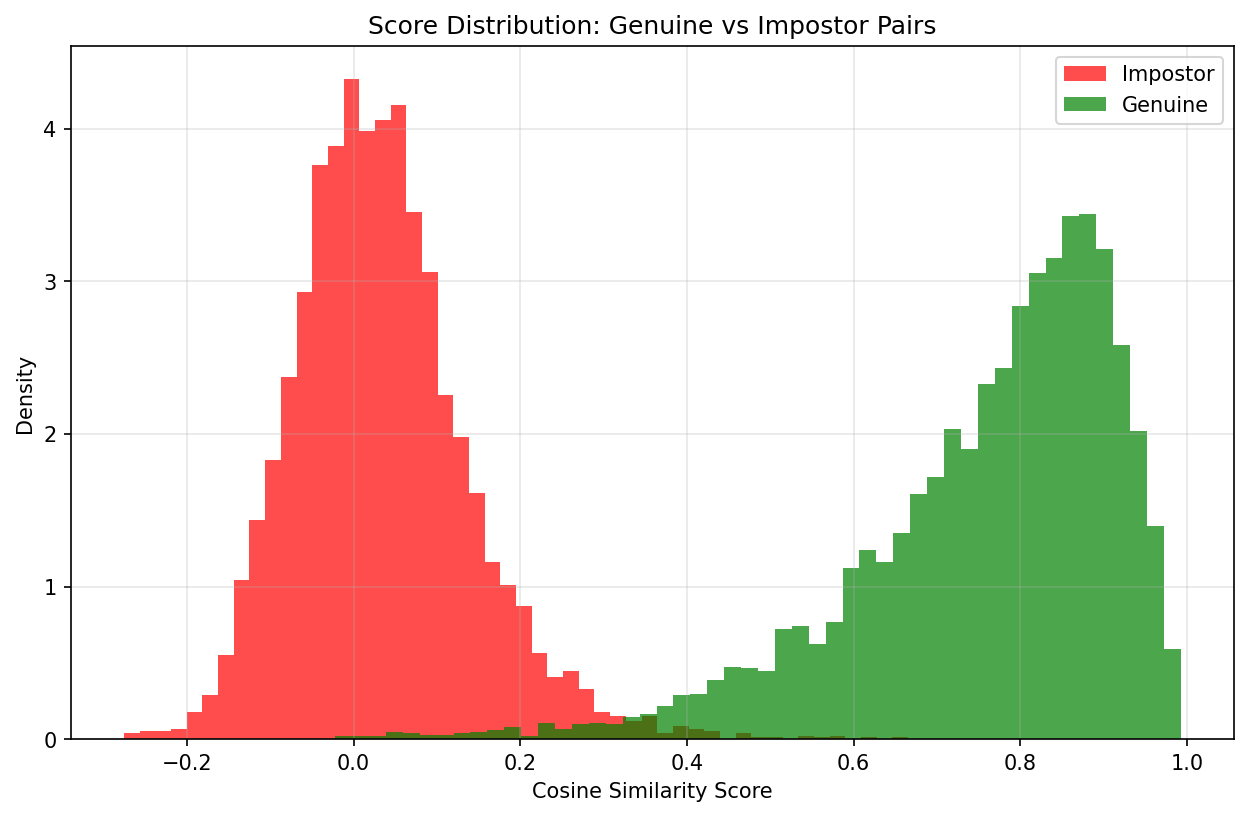
\includegraphics[width=\columnwidth]{score_dist_test.png}
\caption{Genuine (green) vs.\ impostor (red) cosine similarity distributions on the test set. Clear bimodal separation enables reliable verification at $\tau\!\approx\!0.30$.}
\label{fig:scores}
\end{figure}

\begin{figure}[t]
\centering
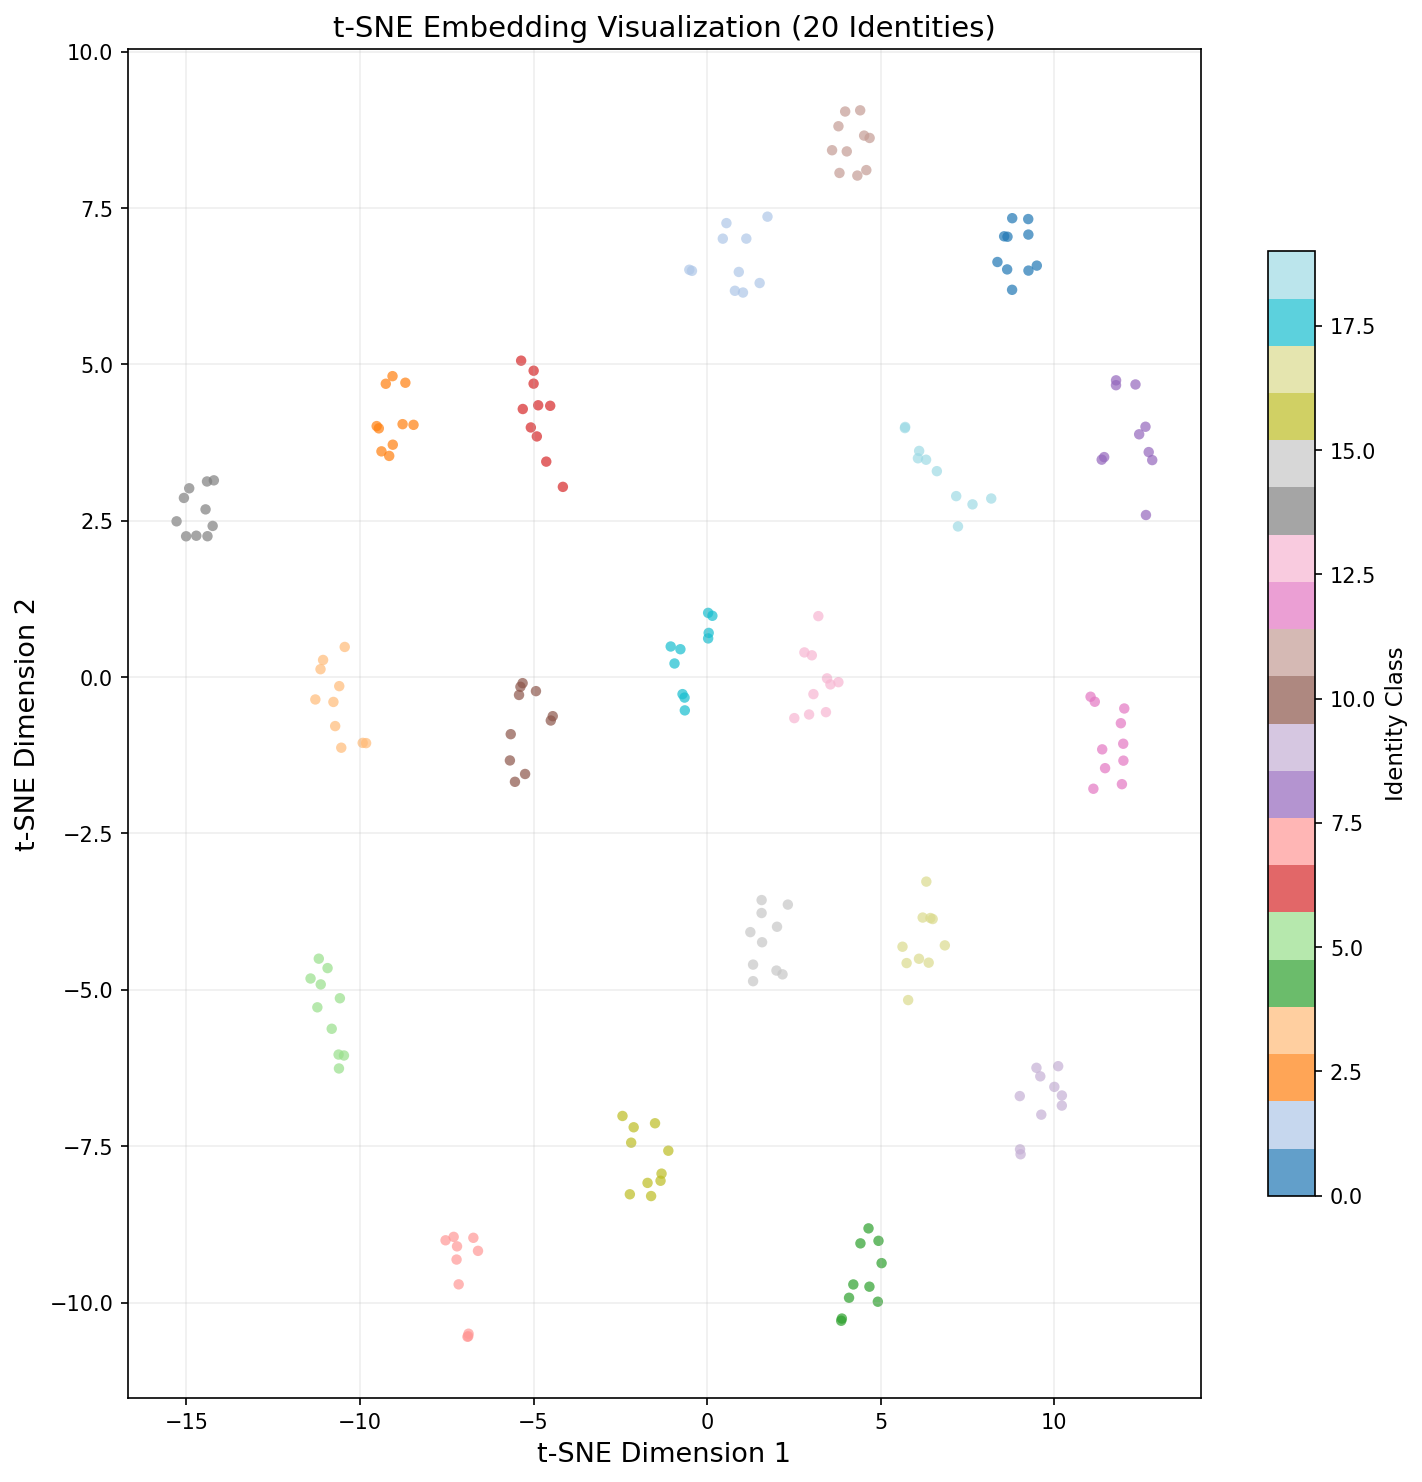
\includegraphics[width=\columnwidth]{tsne_embeddings.png}
\caption{t-SNE visualization of 256-D advanced embeddings for 20 test identities. Tight, well-separated clusters confirm discriminative embedding learning.}
\label{fig:tsne}
\end{figure}

% ============================================================
\section{Preliminary Results and Comparison}

\subsection{Baseline Floor vs.\ Advanced Model}
To quantify the contribution of deep metric learning, we compare the advanced model against a realistic floor: an ImageNet-pretrained ResNet18 \emph{without} palmprint-specific fine-tuning. Features (512-D, L2-normalized) are scored by cosine similarity on the identical test pair set (seed 42). Both systems are evaluated on 5{,}000 genuine and 5{,}000 impostor pairs.

\begin{table}[h]
\centering
\caption{Baseline floor vs.\ advanced model on clean test data.}
\label{tab:compare}
\begin{tabular}{lcc}
\toprule
\textbf{Metric} & \textbf{Pretrained ResNet18} & \textbf{ResNet18 + ArcFace} \\
                & \textbf{(baseline floor)} & \textbf{(advanced)} \\
\midrule
EER              & 6.50\%  & \textbf{1.67\%} \\
FAR @ 1\% FRR    & 28.74\% & \textbf{4.12\%} \\
FAR @ 0.1\% FRR  & 47.52\% & \textbf{48.88\%}$^\dagger$ \\
Genuine $\mu$    & 0.914   & 0.759 \\
Impostor $\mu$   & 0.677   & 0.033 \\
\bottomrule
\multicolumn{3}{l}{\footnotesize $^\dagger$Floor nearly matches at this strict operating point because both}\\
\multicolumn{3}{l}{\footnotesize suffer from overlapping tails; EER and FAR@1\%FRR are the primary metrics.}
\end{tabular}
\end{table}

The advanced model cuts EER by $3.9\times$ (6.50\% $\to$ 1.67\%) and FAR at 1\% FRR by $7.0\times$ (28.74\% $\to$ 4.12\%). The impostor mean drops from 0.677 to 0.033, showing that the ArcFace objective successfully pushes apart the angular positions of different identities on the hypersphere; the pretrained features, by contrast, collapse all palmprint images into a narrow cone of ImageNet-inherited features.

\subsection{ROC and Threshold Analysis}
Fig.~\ref{fig:roc} shows the ROC curve for the advanced model (AUC $>$ 0.99). The EER operating point corresponds to $\tau\!\approx\!0.30$. The high FAR @ 0.1\% FRR (48.88\%) reveals overlapping distribution tails: at very strict operating points required for high-security deployments, the system cannot separate all pairs. This likely stems from limited intra-class variability in training ($\sim$10 images per class), which constrains the model's coverage of within-identity variation.

\begin{figure}[t]
\centering
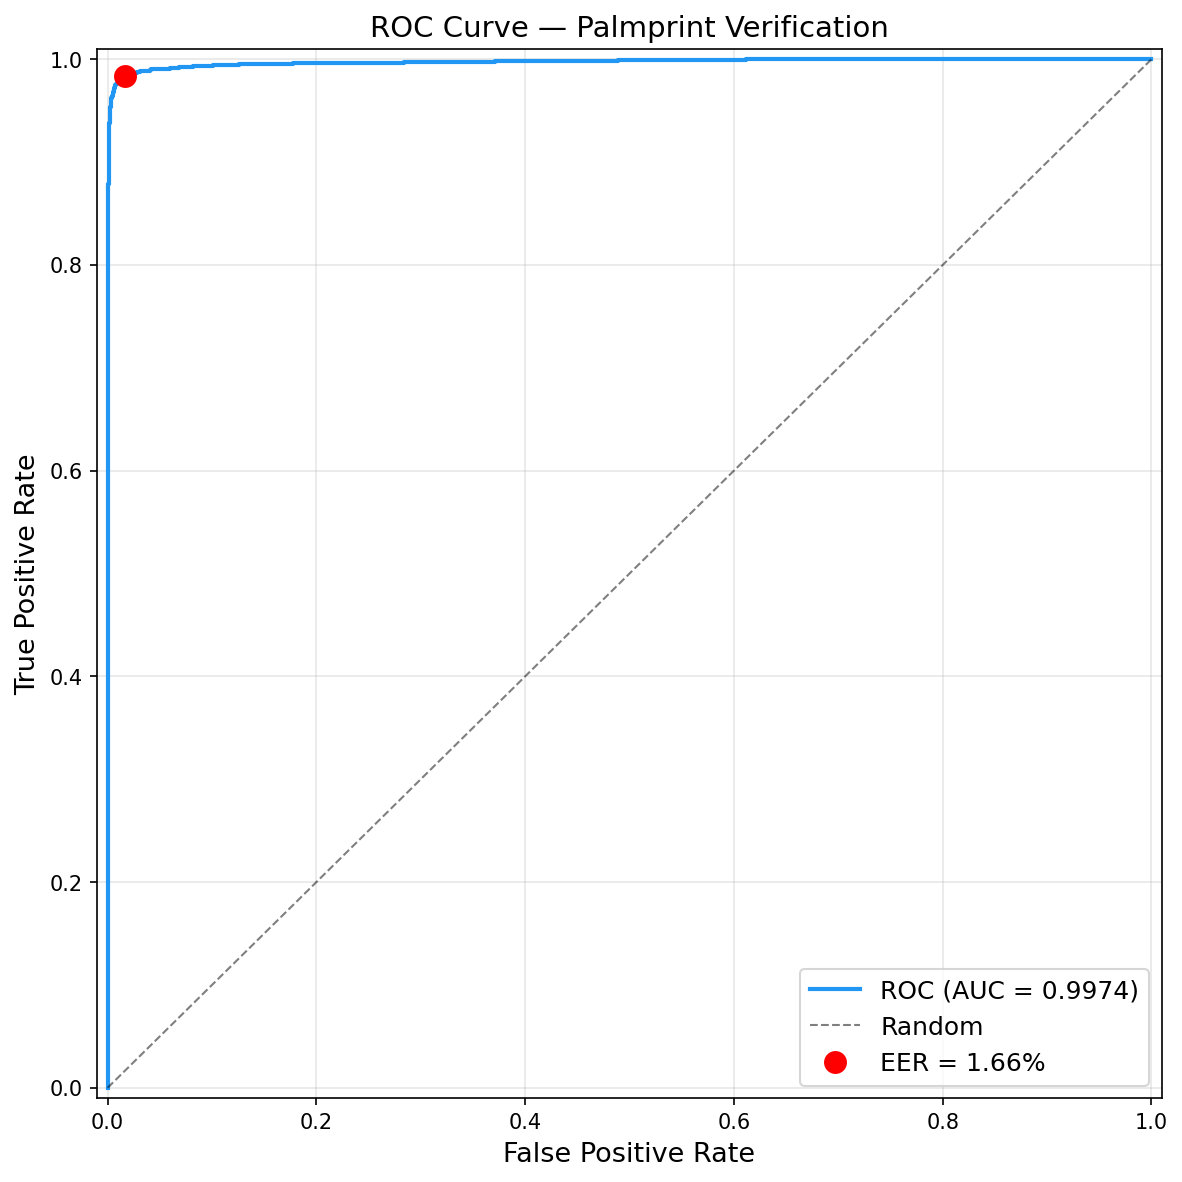
\includegraphics[width=\columnwidth]{roc_curve.png}
\caption{ROC curve of the advanced model with EER operating point (red dot). AUC $>$ 0.99.}
\label{fig:roc}
\end{figure}

\subsection{Robustness Benchmark}
We re-evaluate the advanced model under 9 corruption types at 5 severity levels (45 conditions); corrupted images are generated on the fly from the clean test set and the same 10{,}000 pairs are re-scored. Table~\ref{tab:robustness} ranks corruption types by worst-case degradation relative to the clean EER of 1.67\% (1.72\% measured on the corruption pipeline's clean baseline).

\begin{table}[h]
\centering
\caption{Robustness benchmark on the advanced model: EER degradation by corruption type.}
\label{tab:robustness}
\begin{tabular}{lccc}
\toprule
\textbf{Corruption} & \textbf{Mean EER} & \textbf{Worst EER} & \textbf{Rel.\ Degrad.} \\
\midrule
Motion Blur  & 10.74\% & 19.67\% & +1{,}041\% \\
Noise        & 9.00\%  & 21.90\% & +1{,}170\% \\
Brightness   & 5.45\%  & 15.45\% & +796\%     \\
Occlusion    & 5.29\%  & 7.80\%  & +352\%     \\
Rotation     & 4.52\%  & 9.15\%  & +430\%     \\
JPEG         & 4.19\%  & 11.12\% & +545\%     \\
Gauss.\ Blur & 2.83\%  & 4.45\%  & +158\%     \\
Scale        & 2.75\%  & 3.05\%  & +77\%      \\
Contrast     & 1.85\%  & 2.28\%  & +32\%      \\
\bottomrule
\end{tabular}
\end{table}

\begin{figure}[t]
\centering
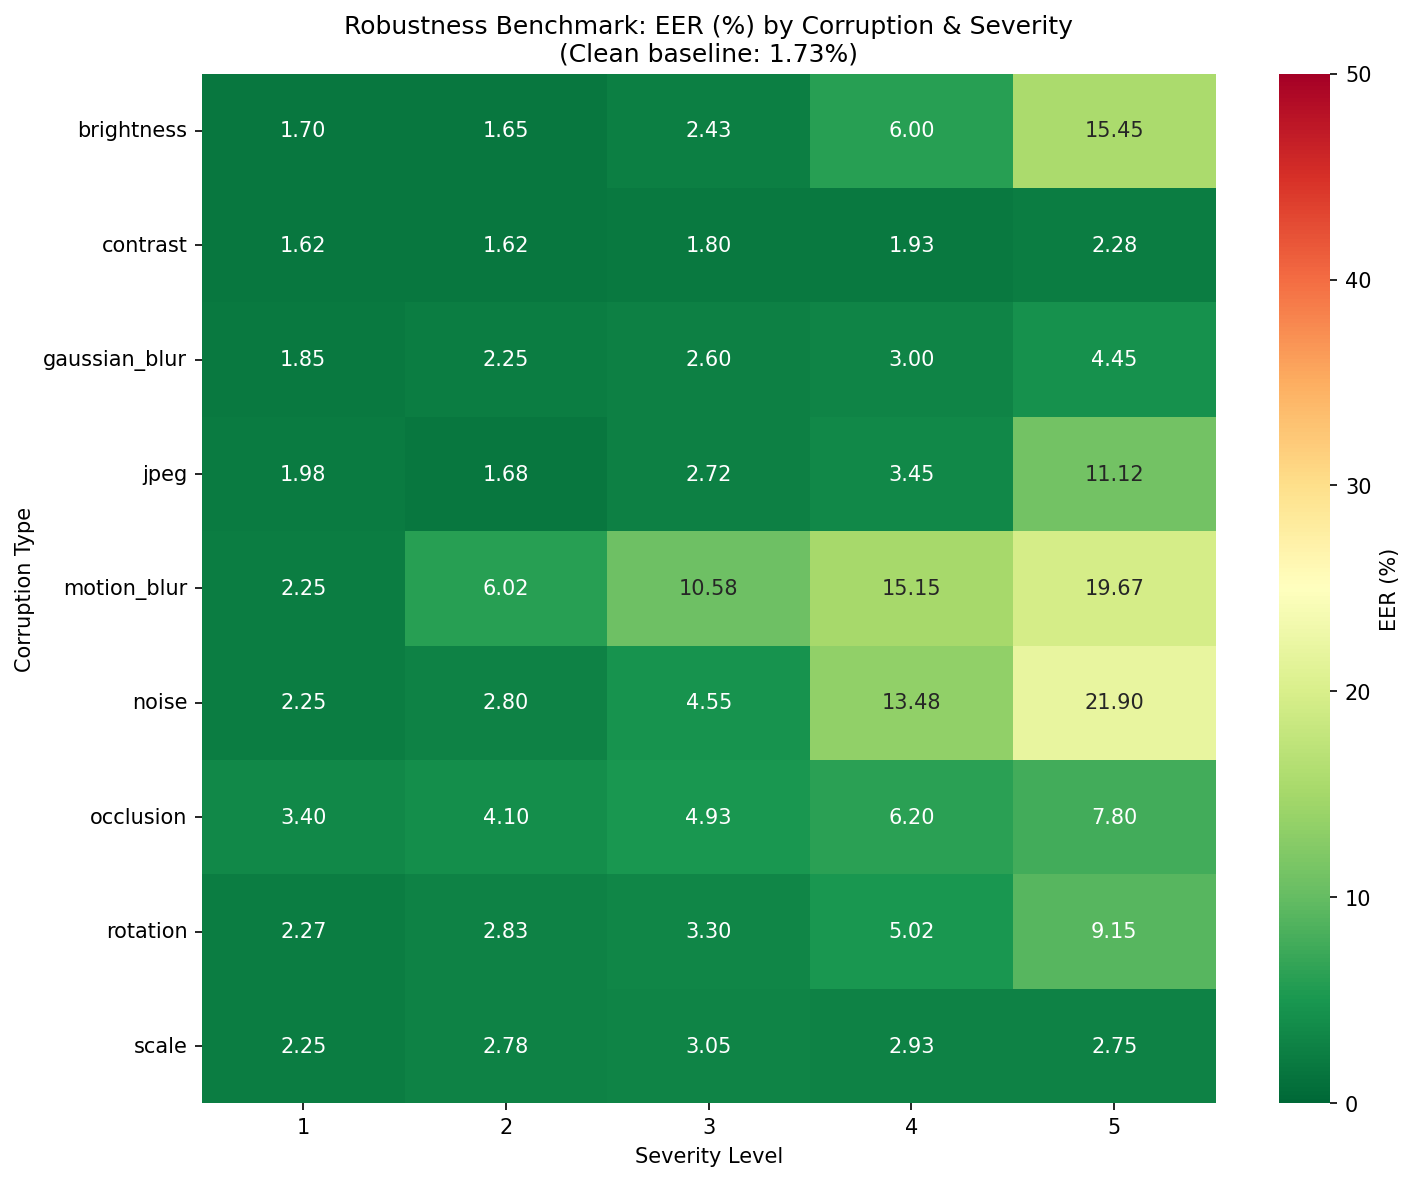
\includegraphics[width=\columnwidth]{eer_heatmap.png}
\caption{Robustness EER heatmap: 9 corruption types $\times$ 5 severity levels. Darker cells indicate higher EER.}
\label{fig:heatmap}
\end{figure}

\begin{figure}[t]
\centering
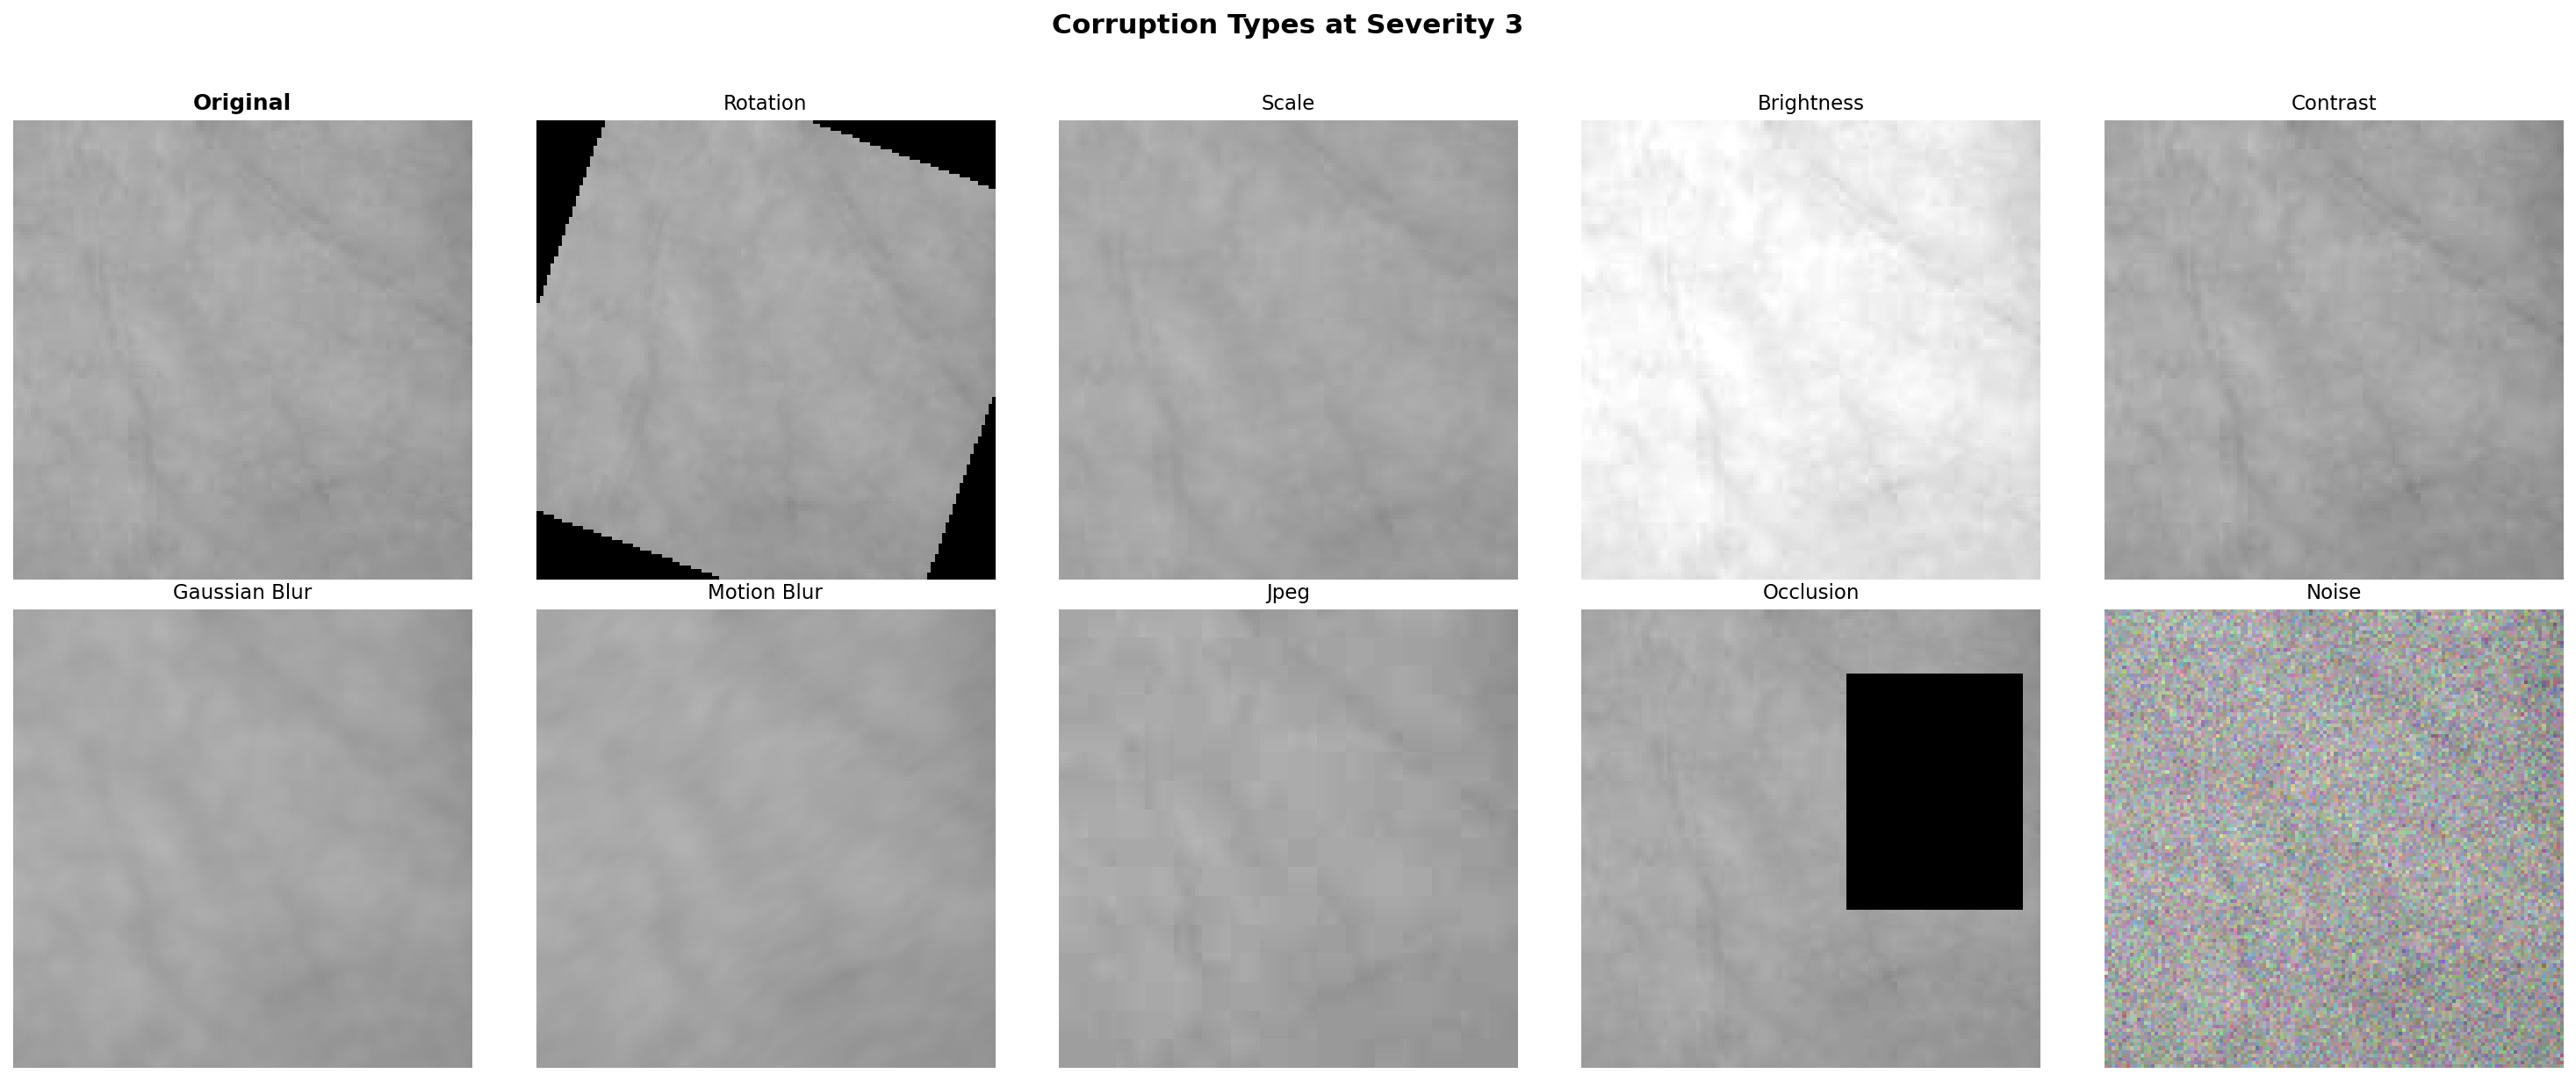
\includegraphics[width=\columnwidth]{corruption_samples.png}
\caption{Original palmprint and 9 corruption types at severity~3. Noise, motion blur, and brightness cause the steepest EER growth at severity~5.}
\label{fig:corruptions}
\end{figure}

\subsection{Error Analysis}
The three worst corruptions---noise (+1{,}170\%), motion blur (+1{,}041\%), and brightness (+796\%)---each drive EER above 15\% at severity~5. The failure mechanism is consistent: these corruptions destroy or mask the fine-grained texture cues (principal lines, wrinkles) that dominate the learned representation. Qualitatively, failure cases concentrate in three regimes: (i) \emph{high-noise probes} where the impostor similarity spikes because Gaussian noise fills the high-frequency band the network relies on, (ii) \emph{motion-blurred genuine pairs} where intra-class similarity collapses toward the impostor mode as line structure is smeared, and (iii) \emph{over-exposed samples} where saturated pixels erase texture entirely. By contrast, contrast changes (+32\%) and scale changes (+77\%) are nearly absorbed---contrast by batch normalization and ImageNet normalization, scale by the training-time random crop and affine augmentation. These asymmetries are the clearest signal for the mitigation phase: a targeted mix of noise/blur/brightness augmentation or a dedicated quality gate should address the dominant failure modes.

% ============================================================
\section{Code Repository}

Source code is at \url{https://github.com/onggiahuy97/cs228-palmprint}.

\medskip
\noindent\textbf{Repository layout:}
\begin{itemize}
    \item \texttt{src/} -- training, evaluation, corruption, baseline, visualization
    \item \texttt{splits/} -- subject-disjoint split definitions (JSON + TXT)
    \item \texttt{figures/} -- ROC, t-SNE, training curves, corruption samples
    \item \texttt{checkpoints/baseline\_v2/} -- advanced model weights, per-epoch snapshots, clean-test logs, \texttt{robustness/} CSVs and plots
    \item \texttt{checkpoints/baseline\_floor/} -- pretrained-only floor \texttt{metrics.json}
    \item \texttt{report/} -- this document
\end{itemize}

\noindent\textbf{Key scripts:}
\begin{itemize}
    \item \texttt{src/train.py} -- ArcFace training loop with early stopping
    \item \texttt{src/evaluate.py} -- verification pair generation + EER/FAR/FRR
    \item \texttt{src/robustness\_eval.py} -- 45-condition corruption benchmark
    \item \texttt{src/baseline\_floor.py} -- pretrained-only ResNet18 baseline
    \item \texttt{src/corruptions.py} -- 9 corruption functions $\times$ 5 severities
    \item \texttt{src/model.py} -- ResNet18 embedder + ArcFace head
\end{itemize}

% ============================================================
\bibliographystyle{IEEEtran}
\begin{thebibliography}{11}

\bibitem{polyu}
PolyU--IITD Contactless Palmprint Database v3.0, The Hong Kong Polytechnic University.

\bibitem{deng2019arcface}
J.~Deng, J.~Guo, N.~Xue, and S.~Zafeiriou, ``ArcFace: Additive angular margin loss for deep face recognition,'' in \textit{Proc. IEEE/CVF CVPR}, 2019, pp.~4690--4699.

\bibitem{he2016deep}
K.~He, X.~Zhang, S.~Ren, and J.~Sun, ``Deep residual learning for image recognition,'' in \textit{Proc. IEEE CVPR}, 2016, pp.~770--778.

\bibitem{hendrycks2019benchmarking}
D.~Hendrycks and T.~Dietterich, ``Benchmarking neural network robustness to common corruptions and perturbations,'' in \textit{Proc. ICLR}, 2019.

\bibitem{schroff2015facenet}
F.~Schroff, D.~Kalenichenko, and J.~Philbin, ``FaceNet: A unified embedding for face recognition and clustering,'' in \textit{Proc. IEEE CVPR}, 2015, pp.~815--823.

\bibitem{zhang2003palmcode}
D.~Zhang, W.-K.~Kong, J.~You, and M.~Wong, ``Online palmprint identification,'' \textit{IEEE Trans. Pattern Anal. Mach. Intell.}, vol.~25, no.~9, pp.~1041--1050, 2003.

\bibitem{kong2004competitive}
A.~W.-K.~Kong and D.~Zhang, ``Competitive coding scheme for palmprint verification,'' in \textit{Proc. ICPR}, 2004, vol.~1, pp.~520--523.

\bibitem{guo2009bocv}
Z.~Guo, D.~Zhang, L.~Zhang, and W.~Zuo, ``Palmprint verification using binary orientation co-occurrence vector,'' \textit{Pattern Recognition Letters}, vol.~30, no.~13, pp.~1219--1227, 2009.

\bibitem{genovese2019palmnet}
A.~Genovese, V.~Piuri, K.~N.~Plataniotis, and F.~Scotti, ``PalmNet: Gabor-PCA convolutional networks for touchless palmprint recognition,'' \textit{IEEE Trans. Inf. Forensics Security}, vol.~14, no.~12, pp.~3160--3174, 2019.

\bibitem{matkowski2020palmprint}
W.~M.~Matkowski, T.~Chai, and A.~W.~K.~Kong, ``Palmprint recognition in uncontrolled and uncooperative environment,'' \textit{IEEE Trans. Inf. Forensics Security}, vol.~15, pp.~1601--1615, 2020.

\bibitem{zhong2019palmprint}
D.~Zhong, X.~Du, and K.~Zhong, ``Decade progress of palmprint recognition: A brief survey,'' \textit{Neurocomputing}, vol.~328, pp.~16--28, 2019.

\end{thebibliography}

\end{document}
